% ============================================================================
%  Text-to-SQL Reference Graph
%  ----------------------------------------------------------------------------
%  A citation / influence graph of 25 papers selected around the `txt2sql`
%  seed collection (Purple, MetaSQL, GAR, Combining SLM+LLM, CATSQL, Athena++).
%
%  Compiled with:  pdflatex main.tex   (TeX Live, tikz + xcolor)
% ============================================================================
\documentclass[11pt,a4paper]{article}

\usepackage[margin=1.6cm]{geometry}
\usepackage{tikz}
\usetikzlibrary{arrows.meta, positioning, backgrounds, calc}
\usepackage[table]{xcolor}
\usepackage{booktabs}
\usepackage{array}
\usepackage{caption}
\usepackage[hidelinks]{hyperref}

% ----------------------------------------------------------------------------
% Research-front colour palette (used both in the diagram and the table)
% ----------------------------------------------------------------------------
\definecolor{cBench}{HTML}{1565C0}   % blue     -- benchmarks & evaluation
\definecolor{cSchema}{HTML}{2E7D32}  % green    -- schema linking / neural parsing
\definecolor{cLLM}{HTML}{EF6C00}     % orange   -- LLM prompting / decomposition / agentic
\definecolor{cRank}{HTML}{6A1B9A}    % purple   -- generate-then-rank / self-correction
\definecolor{cSLM}{HTML}{C62828}     % red      -- SLM-LLM collaboration / open-source
\definecolor{cInd}{HTML}{546E7A}     % blue-grey-- industrial NLIDB systems

\tikzset{
  every node/.style={font=\footnotesize, align=center, inner sep=1.5pt,
                     text width=2.0cm, minimum height=0.78cm, line width=0.5pt},
  bench/.style ={draw=cBench,  fill=cBench!12,  rounded corners=2pt},
  schema/.style={draw=cSchema, fill=cSchema!12, rounded corners=2pt},
  llm/.style   ={draw=cLLM,    fill=cLLM!15,    rounded corners=2pt},
  rank/.style  ={draw=cRank,   fill=cRank!12,   rounded corners=2pt},
  slm/.style   ={draw=cSLM,    fill=cSLM!12,    rounded corners=2pt},
  ind/.style   ={draw=cInd,    fill=cInd!15,    rounded corners=2pt},
  citeedge/.style={-{Stealth[length=2.2mm]}, draw=black!45, line width=0.45pt},
  seednode/.style={line width=1.0pt},
}

\begin{document}

\title{\bf Text-to-SQL: A Reference Graph of 25 Selected Papers}
\author{Automatically assembled from the \texttt{txt2sql} Zotero collection}
\date{\today}
\maketitle

\section{Reference graph}

Figure~\ref{fig:graph} shows the citation / influence relationships among the
25 selected papers. Each node is one paper; the node colour encodes its
research front (legend at the bottom). Directed edges point from a later paper
to the earlier work it cites or builds on. Papers marked with a thicker border
are the six seed papers from the \texttt{txt2sql} collection.

\begin{figure}[!htbp]
\centering
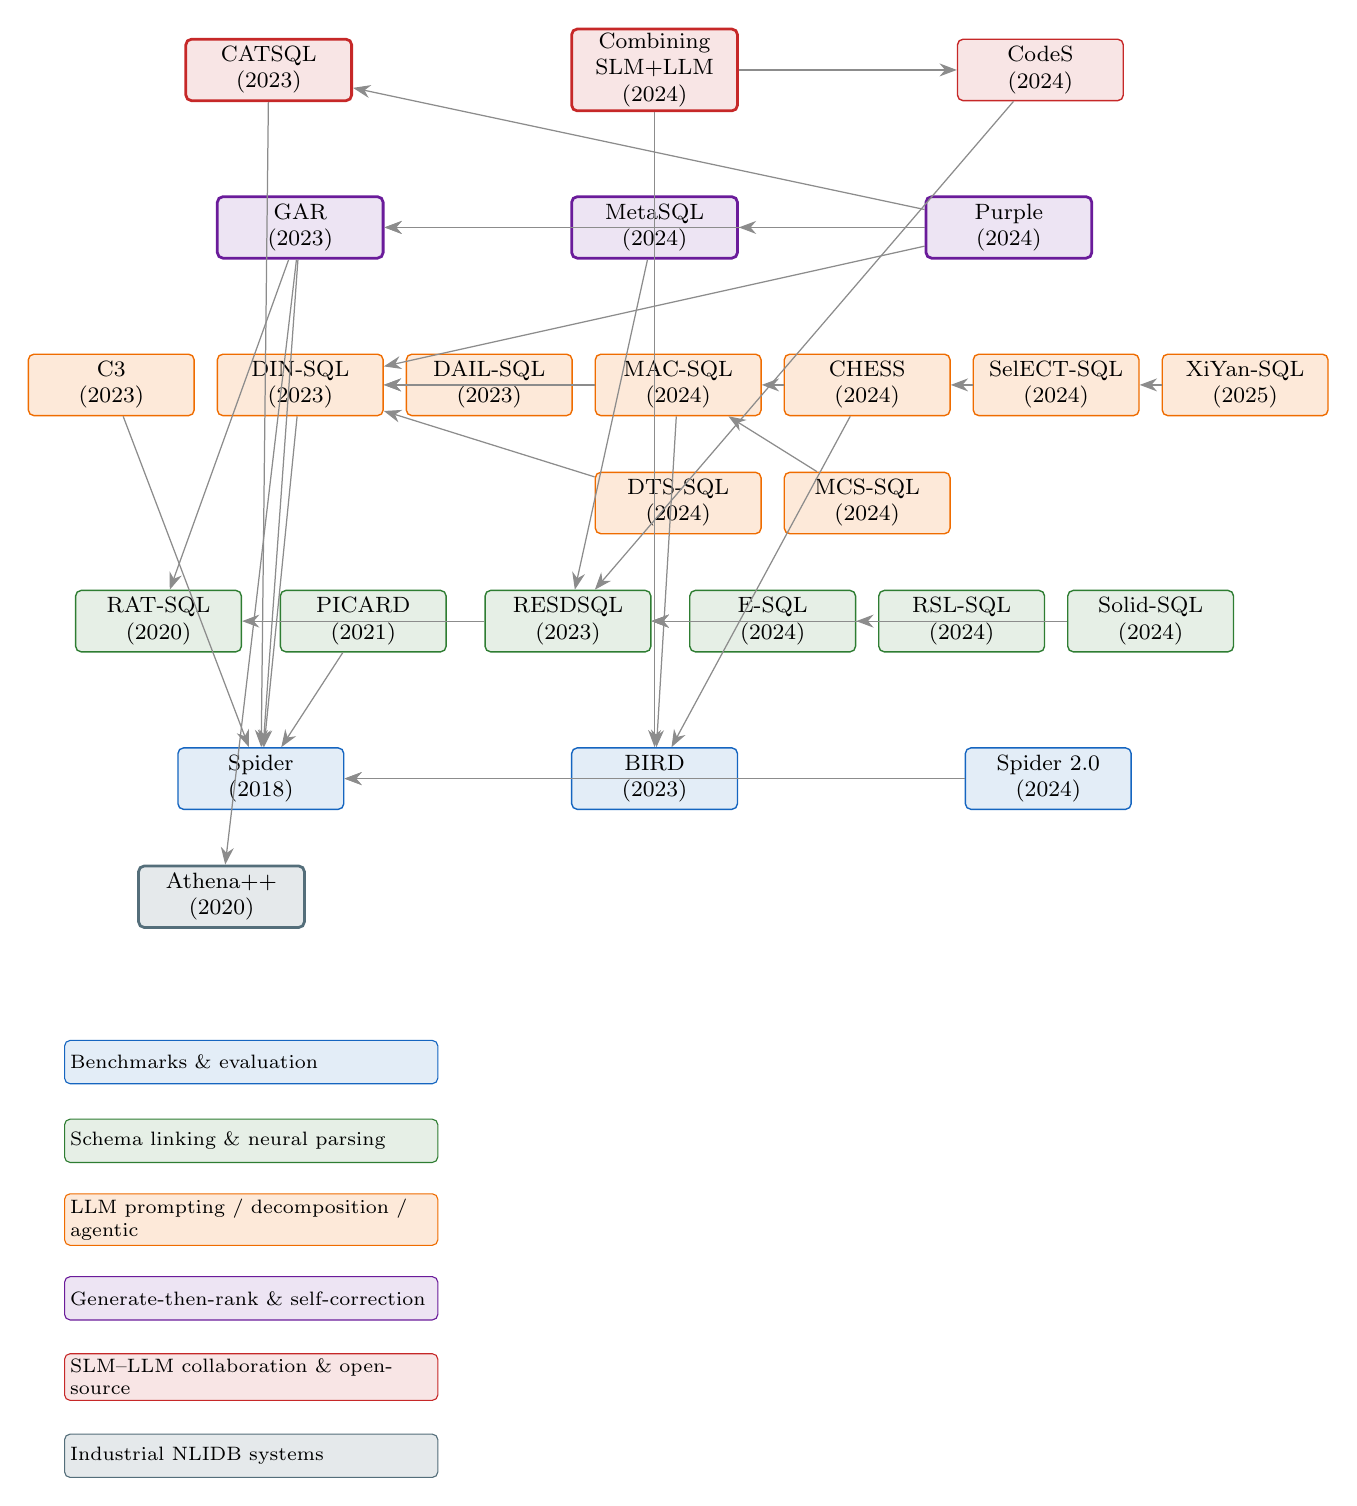
\begin{tikzpicture}[x=1.0cm, y=1.0cm]

% ================================================================
% Node positions (lanes = research fronts, roughly left->right = time)
% ================================================================

% --- Lane 6: Industrial NLIDB systems (blue-grey) ---------------------------
\node[ind, seednode] (athena) at (2.0, -0.5) {Athena++\\(2020)};

% --- Lane 5: Benchmarks & evaluation (blue) ---------------------------------
\node[bench] (spider)  at (2.5, 1.0)  {Spider\\(2018)};
\node[bench] (bird)    at (7.5, 1.0)  {BIRD\\(2023)};
\node[bench] (spider2) at (12.5,1.0)  {Spider 2.0\\(2024)};

% --- Lane 4: Schema linking & neural parsing (green) ------------------------
\node[schema] (ratsql)   at (1.2, 3.0)  {RAT-SQL\\(2020)};
\node[schema] (picard)   at (3.8, 3.0)  {PICARD\\(2021)};
\node[schema] (resdsql)  at (6.4, 3.0)  {RESDSQL\\(2023)};
\node[schema] (esql)     at (9.0, 3.0)  {E-SQL\\(2024)};
\node[schema] (rslsql)   at (11.4,3.0)  {RSL-SQL\\(2024)};
\node[schema] (solidsql) at (13.8,3.0)  {Solid-SQL\\(2024)};

% --- Lane 3: LLM prompting / decomposition / agentic (orange) ---------------
\node[llm] (c3)        at (0.6, 6.0)  {C3\\(2023)};
\node[llm] (dinsql)    at (3.0, 6.0)  {DIN-SQL\\(2023)};
\node[llm] (dailsql)   at (5.4, 6.0)  {DAIL-SQL\\(2023)};
\node[llm] (macsql)    at (7.8, 6.0)  {MAC-SQL\\(2024)};
\node[llm] (chess)     at (10.2,6.0)  {CHESS\\(2024)};
\node[llm] (selects)   at (12.6,6.0)  {SelECT-SQL\\(2024)};
\node[llm] (xiyansql)  at (15.0,6.0)  {XiYan-SQL\\(2025)};
\node[llm] (dtssql)    at (7.8, 4.5)  {DTS-SQL\\(2024)};
\node[llm] (mcssql)    at (10.2,4.5)  {MCS-SQL\\(2024)};

% --- Lane 2: Generate-then-rank / self-correction (purple) ------------------
\node[rank, seednode] (gar)     at (3.0, 8.0)  {GAR\\(2023)};
\node[rank, seednode] (metasql) at (7.5, 8.0)  {MetaSQL\\(2024)};
\node[rank, seednode] (purple)  at (12.0,8.0)  {Purple\\(2024)};

% --- Lane 1: SLM-LLM collaboration / open-source (red) ----------------------
\node[slm, seednode] (catsql)    at (2.6, 10.0) {CATSQL\\(2023)};
\node[slm, seednode] (combining) at (7.5, 10.0) {Combining SLM+LLM\\(2024)};
\node[slm] (codes)               at (12.4,10.0) {CodeS\\(2024)};

% ================================================================
% Citation / influence edges (later -> earlier)
% ================================================================

% Benchmark spine
\draw[citeedge] (bird)    -- (spider);
\draw[citeedge] (spider2) -- (spider);

% Schema-linking lineage
\draw[citeedge] (picard)  -- (spider);
\draw[citeedge] (resdsql) -- (ratsql);
\draw[citeedge] (esql)    -- (resdsql);
\draw[citeedge] (rslsql)  -- (resdsql);
\draw[citeedge] (solidsql)-- (resdsql);
\draw[citeedge] (solidsql)-- (esql);

% LLM prompting / decomposition / agentic lineage
\draw[citeedge] (c3)      -- (spider);
\draw[citeedge] (dinsql)  -- (spider);
\draw[citeedge] (dailsql) -- (dinsql);
\draw[citeedge] (macsql)  -- (dinsql);
\draw[citeedge] (macsql)  -- (bird);
\draw[citeedge] (chess)   -- (macsql);
\draw[citeedge] (chess)   -- (bird);
\draw[citeedge] (dtssql)  -- (dinsql);
\draw[citeedge] (mcssql)  -- (macsql);
\draw[citeedge] (selects) -- (chess);
\draw[citeedge] (xiyansql)-- (selects);

% Generate-then-rank lineage
\draw[citeedge] (gar)     -- (spider);
\draw[citeedge] (gar)     -- (ratsql);
\draw[citeedge] (gar)     -- (athena);
\draw[citeedge] (metasql) -- (gar);
\draw[citeedge] (metasql) -- (resdsql);
\draw[citeedge] (purple)  -- (metasql);
\draw[citeedge] (purple)  -- (gar);
\draw[citeedge] (purple)  -- (dinsql);
\draw[citeedge] (purple)  -- (catsql);

% SLM-LLM collaboration / open-source lineage
\draw[citeedge] (catsql)    -- (spider);
\draw[citeedge] (combining) -- (codes);
\draw[citeedge] (combining) -- (bird);
\draw[citeedge] (codes)     -- (resdsql);

% ================================================================
% Legend
% ================================================================
\begin{scope}[every node/.style={font=\scriptsize, align=left, inner sep=2pt,
      text width=4.6cm, minimum height=0.55cm}]
\node[bench, anchor=west]  at (0, -2.6) {Benchmarks \& evaluation};
\node[schema,anchor=west]  at (0, -3.6) {Schema linking \& neural parsing};
\node[llm, anchor=west]    at (0, -4.6) {LLM prompting / decomposition / agentic};
\node[rank, anchor=west]   at (0, -5.6) {Generate-then-rank \& self-correction};
\node[slm, anchor=west]    at (0, -6.6) {SLM--LLM collaboration \& open-source};
\node[ind, anchor=west]    at (0, -7.6) {Industrial NLIDB systems};
\end{scope}

\end{tikzpicture}
\caption{Reference graph of the 25 selected text-to-SQL papers.
Colours denote research fronts; arrows denote citations / influence
(directed from the later paper to the earlier paper it builds on).
Thick-bordered nodes are the six seed papers.}
\label{fig:graph}
\end{figure}

% ============================================================================
\section{Papers grouped by research front}
% ============================================================================

\begin{table}[!htbp]
\centering
\caption{The 25 selected papers grouped by research front. Seed papers are
marked with $\dagger$.}
\label{tab:fronts}
\renewcommand{\arraystretch}{1.35}
\begin{tabular}{>{\raggedright\arraybackslash}p{5.4cm}
                >{\raggedright\arraybackslash}p{11.6cm}}
\toprule
\textbf{Research front (colour)} & \textbf{Papers} \\
\midrule
\rowcolor{cBench!10}
Benchmarks \& evaluation (blue)
  & Spider (2018, EMNLP); BIRD (2023, NeurIPS D\&B); Spider 2.0 (2024/ICLR~2025) \\
\rowcolor{cSchema!10}
Schema linking \& neural parsing (green)
  & RAT-SQL (2020, ACL); PICARD (2021, EMNLP); RESDSQL (2023, AAAI);
    E-SQL (2024, arXiv:2409.16751); RSL-SQL (2024, arXiv:2411.00073);
    Solid-SQL (2024, arXiv:2412.12522) \\
\rowcolor{cLLM!10}
LLM prompting / decomposition / agentic (orange)
  & C3 (2023, arXiv:2307.07306); DIN-SQL (2023, NeurIPS);
    DAIL-SQL (2023, arXiv:2308.15363); MAC-SQL (2024, NAACL);
    CHESS (2024, arXiv:2405.16755); DTS-SQL (2024, arXiv:2402.01117);
    MCS-SQL (2024, arXiv:2405.07467); SelECT-SQL (2024, arXiv:2409.10007);
    XiYan-SQL (2025, arXiv:2507.04701) \\
\rowcolor{cRank!10}
Generate-then-rank \& self-correction (purple)
  & GAR (2023, ICDE)$\dagger$; MetaSQL (2024, ICDE)$\dagger$;
    Purple (2024, ICDE)$\dagger$ \\
\rowcolor{cSLM!10}
SLM--LLM collaboration \& open-source models (red)
  & CATSQL (2023, VLDB)$\dagger$; Combining SLM+LLM (2024, VLDB)$\dagger$;
    CodeS (2024, SIGMOD) \\
\rowcolor{cInd!10}
Industrial NLIDB systems (blue-grey)
  & Athena++ (2020, VLDB)$\dagger$ \\
\bottomrule
\end{tabular}
\end{table}

\section{Composition summary}

The graph contains \textbf{25 papers}: the 6 seed papers plus 19 papers
discovered by backward (reference) and forward (citation) search. Of the 19
newly added papers, 11 are published in 2024 or later (58\%), covering the
2024--2025 frontier of LLM-based text-to-SQL (multi-agent pipelines, schema
linking for LLMs, ensemble/selection decoding, and open-source models), while
the remaining 8 anchor the field's benchmarks and pre-LLM neural parsers.

\end{document}
